\chapter{Electromagnetic Worldlines - Numerical Methods and Results}
\label{ch:numerical}

The goal of this project is to build a general numerical method for computing 
Casimir energies.  As a first step, it is necessary to test the proposed methods in well understood 
cases, such as for planar media.  We have developed numerical methods that should allow efficient computations in the general
case, despite emphasizing planar media in these calculations.  In a general geometry, these methods 
could still be applied to describe scalar fields coupled to a dielectric, that could serve 
as an uncontrolled approximation to the full EM field.
%  Despite the emphasis on planar geometries,
% we have tried to develop methods that would be well suited to more complicated geometries,
% and test them in the simple geometry.  In this case we can carefully test their convergence properties
% as the path resolution is increased. 

Even in a planar geometry a number of tools are required to make the electromagnetic worldline methods tractable.
The TM polarization is challenging, and has prompted most of these developments.
The same developments have been used to enhance the TE polarization methods, and could be applied to improve existing Dirichlet
worldline methods.

The primary ingredients for the numerical methods are ways of efficiently 
constructing Brownian paths and a technique for Monte Carlo sampling of the path starting points $x_0$
and path time $\cT$.  In the case of the TE polarization, these are all quite straightforward.  
However, the simplest numerical estimates of the TM Casimir energy have a large variance which
grows as the path length $N$ is increased.  Those numerical fluctuations can be tempered by changing the methods
used to construct the paths.  In addition, the TM Casimir--Polder energy involves spatial derivatives of the worldline path integral.

The numerical results will be compared against the expected analytical results.
The worldline method tends to straightforwardly reproduce the expected distance dependence due to the
integration over $\cT$, as was briefly discussed in Sec.~\ref{sec:worldline_distance_dep}. 
That is still true within the context of electromagnetic worldlines. 
All of the simulations are carried out for a non-dispersive media at zero temperature.
At the end we will suggest how to generalize the calculations to include dispersion.  

(The numerical results on the TE Casimir energies were published in Ref.~\cite{Mackrory2016}.
A manuscript discussing the gradient estimations presented here and in the next chapter is in
preparation, and the TM results and methods will also be published.)

\section{TE Casimir Numerics}

In this section we will discuss numerically calculating the TE Casimir and Casimir--Polder energies 
from the worldline expressions in Eqs.~(\ref{eq:TE_Casimir}) and (\ref{eq:TE_Casimir_Polder}).
We will first discuss generating the paths, sampling starting positions $\vect{x}_0$ and path times $\cT$,
and evaluating the dielectric path average $\langle \epsr\rangle$.
 % Despite working with expressions adapted to planar
% media, we will endeavour to develop general purpose numerical methods that would work in more general
% geometries.  
% Recall that the Casimir energy~(\ref{eq:TE_Casimir}) is
% \begin{equation}
%   E\subTE-E\sup0 = -\frac{\hbar c}{2(2\pi)^{D/2}}\int_0^\infty\frac{d\cT}{\cT^{1+D/2}}\int d\vect{x}_0
%   \biggdlangle
%   \frac{1}{\sqrt{\langle \epsrab\rangle}}-\frac{1}{\sqrt{\epsrab(\vect{x}_0)}}\biggdrangle_{x(t)},
% \end{equation}
% where we have momentarily suppressed the renormalization from subtracting off the single body
% energies.    

\subsection{Path Generation}

The principal element of the worldline method is evaluating a potential along an ensemble of Gaussian
paths.  This allows the $N$-dimensional integral over positions to be efficiently evaluated in a 
Monte Carlo fashion by generating an ensemble of Brownian bridges.
It is of primary importance to be able to efficiently generate these Gaussian sample paths. 

\subsubsection{Open Brownian Bridges: V-loop Construction}


% The v-loop algorithm is derived by decoupling the product of $N$ Gaussian probability densities 
% into $N-1$ independent Gaussian deviates.
Since the numerical methods will require open and closed Brownian bridges of fixed length $N$, 
we will derive the ``v-loop'' algorithm for generating open paths~\cite{Gies2003}.   
For open paths the starting and end points $x_0$ and $x_N$ differ, while for closed paths $x_N=x_0$
Consider a Gaussian density of $N$ steps in one dimension, where the end points $x_0$ and $x_N$ 
are fixed:
\begin{equation}
  P(x_1,\ldots,x_{N-1}) = (2\pi\Delta\cT)^{-N/2}\exp\left[-\sum_{j=0}^{N-1}\frac{(x_{j+1}-x_j)^2}{2\Delta\cT}\right].
  \label{eq:Gaussian_distrib}
\end{equation}
It is convenient to define shifted, normalized variables $y_k = (x_k-x_0)/\sqrt{\Delta \cT}$.
The exponent for the product of coupled Gaussians then involves the sum
\begin{equation}
\frac{y_1^2}{2}+\frac{(y_2-y_1)^2}{2}+\cdots+\frac{(y_{N-1}-y_{N-2})^2}{2}+\frac{(\Delta y-y_{N-1})^2}{2},
\label{eq:Xexp}
\end{equation}
where $\Delta y :=(x_N-x_0)/\sqrt{\Delta \cT}$.  
The exponent~(\ref{eq:Xexp}) can be decoupled by completing the square repeatedly,
starting at $y_{N-1}$.
The two terms of the sum involving $y_{N-1}$ can be rewritten as
\begin{align}
  & \frac{(y_{N-1}-\Delta y)^2}{2\sigma_{N-1}^2}+\frac{(y_{N-1}-y_{N-2})^2}{2} \nonumber \\
  &= \frac{\sigma^2_{N-1}+1}{2\sigma_{N-1}^2}
  \left(y_{N-1} - \frac{\sigma_{N-1}^2y_{N-2}+\Delta y}{\sigma_{N-1}^2+1}\right)^2 
+ \frac{(y_{N-2}-\Delta y)^2}{2(\sigma^2_{N-1}+1)},\label{eq:decouple_barf}
  % &= \frac{1}{2c_{N-1}}
  % \left(y_{N-1} - c_{N-1}y_{N-2}-\frac{\Delta y}{\sigma_{N-1}^2+1}\right)^2 + \frac{(y_{N-2}-\Delta x)^2}{2(\sigma^2_{N-1}+1)}\\
\end{align}
where $\sigma^2_{N-1}:=1$, $\sigma^2_{N-2}:=\sigma_{N-1}+1$, and $c_{N-1} = \sigma_{N-1}^2/(\sigma_{N-1}^2+1)$.
%It is possible to quickly develop recursion relations for how the resulting variables transform.  
After each completion of the square, the variance changes to $\sigma^2_{N-j}\rightarrow \sigma^2_{N-j1}+1=j+1$, with the algebra
taking the same form as Eq.~(\ref{eq:decouple_barf}) with the label indices decreasing by one.
Once the process has been repeated $N-1$ times
the exponent becomes 
\begin{equation}
  \frac{\Delta x^2}{2N} + \sum_{j=1}^{N-1} \frac{z_j^2}{2},
\end{equation}
where 
\begin{equation}
  z_j := \frac{1}{c_j}\left(y_j - c_jy_{j-1}-\frac{\Delta x}{N-j+1}\right)^2,\label{eq:zj}
\end{equation}
and 
\begin{equation}
  c_j = \frac{N-j}{N-j+1}.
\end{equation}
The probability distribution~(\ref{eq:Gaussian_distrib}) is then
\begin{equation}
  P(z_1,\ldots z_{N-1}) = \frac{1}{\sqrt{2\pi\cT}}e^{-(x_0-x_{N})^2/(2\cT)}
  \prod_{k=1}^{N-1} \frac{e^{-z_k^2/2}}{\sqrt{2\pi}},
\end{equation}
which accounts for the Jacobian determinant $\prod_{j}\sqrt{c_j}=N^{-1/2}$ from changing variables.
The $z_j$ are independent, standard normal variables.  Once the $z_j$ have been sampled,  
definition~(\ref{eq:zj}) can be inverted to find the coordinates:
\begin{equation}
  x_k = x_0 + \frac{x_N-x_0}{N-k+1}+c_kx_{k-1} + \sqrt{c_k\Delta\cT}z_k.\label{eq:open_vloop}
\end{equation}
This recursion formula shows how to construct a discrete representation for a Brownian bridge from $x_0\rightarrow x_N$ in time $\cT$.
%This normalization is also the normalization factor derived in Eq.~\ref{eq:Gaussian_normalization}.
The integral of the probability density~(\ref{eq:Gaussian_distrib}) could be rewritten as
\begin{equation}
  I = \int \prod_{j=1}^{N-1}dx_j P(x_1,\ldots,x_{N-1})f(x_1,\ldots,x_N)
  = \frac{e^{-\frac{(x_0-x_N)^2}{2\cT}}}{\sqrt{2\pi \cT}}\dlangle f\drangle_{x(t)},
\end{equation}
where the ensemble average is taken over open Brownian bridges between $x_0$ and $x_N$.
The limit of closed paths can be taken by setting $x_N-x_0=0$.
The v-loop construction is also straightforwardly generalized to multi-dimensional Brownian bridges.  
This recursion procedure~(\ref{eq:open_vloop}) also allows the generation of a unit loop for $\cT=1$, which can then be integrated over
multiple starting points $x_0$ and total path times $\cT$.  A closed unit Brownian bridge can be constructed 
via
\begin{equation}
  B_k = c_kB_{k-1} + \sqrt{\frac{c_k}{N}}z_k,\qquad B_0=0, k=1,\ldots,N-1 \label{eq:unit_vloop}
\end{equation}
and a shifted, scaled Brownian bridge can then be constructed as
\begin{equation}
  x_k = x_0 + \sqrt{\cT} B_k,
\end{equation}
where $x_0$ is the shifted starting position of the path, and $\cT$ is the path time.

The v-loop constructed here has an advantage over other methods of generating Brownian bridges, since it only needs to keep 
track of the current position $x_k$ and index $k$ to develop a Brownian bridge.  Other methods such as pro-rated Brownian motion~(\ref{eq:prorate-loop})
or ``d-loops'' (which start with a coarse path, and then refine it by doubling the number of points~\cite{Gies2005})
require knowledge of the whole Brownian motion.  

The original v-loop algorithm used centered paths, where the average position $\langle x\rangle$ is subtracted from the path~\cite{Gies2003}.
This requires first constructing the Brownian bridge, and then subtracting off the mean position.  
This is inconvenient if the path is being generated on the fly 
without storage, or if there are stochastic elements to path construction.  % However it is slightly 
% more adapted to computing Casimir energies. 
In Casimir--Polder applications (or when computing the stress-energy tensor~\cite{Schafer2016}),
 it is preferable to consider paths emanating from a single point $\vect{x}_0$.
  The starting point corresponds to the atom's location, or the point where
the stress-energy tensor is being computed.  

\subsection{Monte Carlo Sampling}

To evaluate the Casimir energy it is necessary to take an ensemble average over many path realizations,
at all starting positions $\vect{x}_0$ and path times $\cT$.  
The original Gies\etal computations emphasized computing the $\cT$ and $\vect{x}_0$ integrals for each path~\cite{Gies2003}.
For Dirichlet worldlines, the path integrand is either zero or one based on whether the path intersects
all of the bodies.  This makes evaluating these integrals a tractable problem, since 
it only requires finding the set of times $\{\cT_k\}$ when paths enter the body, and evaluating 
$\int d\cT\,\cT^{-(1+D/2)}$ during those  times the integral is nonzero.
For example, in their paper computing forces in a sphere-plane geometry, Weber and Gies found analytical
expressions in terms of $\vect{x}_0$ and $\cT$ for when each random path will intersect both bodies~\cite{Weber2010}.
The remaining integrals over $\vect{x}_0$ and $\cT$ were then evaluated on a path-wise basis.

However, for the dielectric integrands of the TE and TM path integrals, 
the integrand varies based on the number of points that are inside the surface.
 For a path of length $N$, this direct method would becomes impractical for large $N$, 
as a large computational effort  must be expended on even a single path.  
%This becomes even more burdensome once the integral over the starting position is accounted for.

Since the $N$-fold integral over positions is being handled in a Monte Carlo fashion, it makes sense to 
treat the remaining integrals over the starting position $\vect{x}_0$ and path times $\cT$ in the same manner.
Each path can be evaluated for a single pair of $\vect{x}_0, \cT$ picked from suitable
distributions.  This is a form of importance sampling, which 
is a powerful tool for accelerating Monte Carlo numerical computations~\cite{Asmussen2007, Glasserman2004}.
This style of importance sampling goes beyond just using the Gaussian probability density to evaluate the 
spatial integrals over the intermediate positions $\vect{x}_k$.  In this case, the importance sampling
relies on estimating which positions and times are likely to contribute the most to the integral. 
This Monte Carlo sampling of $x_0$ and $\cT$ extends the number of independent paths that can be averaged
in a given time, since effort is not wasted on multiple computations on a single path.  

\subsubsection{Sampling Path-Times from a Power Law}

The simplest method of sampling path times is to exploit the $\cT^{-(1+D/2)}$ factor in the integral.
For a particular path, the renormalized TE integrand is only non-zero after the path touches all of the bodies,
which occurs at some path time $\cT_0$.\footnote{For a Brownian motion $\vect{x}(t)$,
the term ``first-touching time'' is reserved for the first time $t_0$ along a path that a Brownian bridge intersects a surface: $\vect{x}(t_0)=d$. 
This is distinct from the first path time $\cT$ when the scaled path intersects a surface.
}
For $\cT>\cT_0$,  the extent of the path grows as $\sqrt{\cT}$, so the integrand $(\langle\epsr\rangle^{-\alpha}-1)$ 
increases as more points enter the bodies.  
However, the $\cT^{-(1+D/2)}$ factor decreases the contributions from large $\cT$.
These facts suggest sampling $\cT$ from a probability distribution 
\begin{equation}
  P(\cT;\cT_0,m)= \frac{(m-1) \cT_0^{m-1}}{\cT^m}\Theta(\cT-\cT_0),\label{eq:Tpower_law}
\end{equation}
where $m>1$ and $\cT_0>0$.  Sampling from this distribution requires being able to estimate the value of $\cT_0$
for each path.  
For the example of paths starting between parallel planes, 
\begin{equation}
  \cT_0=\text{min}\bigg[\left(\frac{-d_1-x_0}{B_-}\right)^2,  \left(\frac{d_2-x_0}{B_+}\right)^2\bigg]
\end{equation}
where $d_1<x_0<d_2$, and $B_\pm$ are the maximum and minimum points
of the unit Brownian path.  The path time $\cT_0$ is the minimum value of $\cT$ such that the path will touch the relevant bodies,
as required to contribute to the energy.
In computing Casimir interaction energies, the path must touch \emph{all} of the bodies, while in Casimir--Polder
calculations, the path must touch \emph{any} of the bodies to contribute.  

Samples from the distribution~(\ref{eq:Tpower_law}) can be generated by inverting the cumulative probability distribution.
(Inversion is a general purpose method of generating random deviates from a given distribution~\cite{NumRecipe}.)
In this case, the inversion requires solving
\begin{equation}
  u=(m-1) \cT_0^{m-1}\int_{\cT_0}^\cT dt\, t^{-m},\label{eq:Tsamp}
\end{equation}
where $u\in [0,1)$ is a uniform random number and $\cT$ is the desired deviate.    
Eq.~(\ref{eq:Tsamp} can be easily solved, with the result that
\begin{align}
%  r&=(m-1) \cT_0^{m-1}\frac{1}{m-1}\left(\frac{1}{\cT_0^{m-1}}-\frac{1}{\cT^{m-1}}\right)\\
%  \left(\frac{\cT_0}{\cT}\right)^{m-1}&= (1-r)\\
 \cT= \frac{\cT_0}{(1-u)^{1/(m-1)}}.
\end{align}
The lower-bound $\cT_0$ can be easily found in simple geometries on a path-wise basis. Random deviates
$\cT$ can then be generated for each path, and each path is then guaranteed to contribute.  

% In a more complicated arrangement of bodies, the lower-bound $\cT_0$ could be found via root-finding,
% to find the minimum path time such that the path touches all of the relevant bodies.  It is important for 
% $\cT_0$ to be a lower bound on the first time the integrand is nonzero, otherwise this method will miss 
% part of the integral.  However, $\cT_0$ should not be set too low, as otherwise numerous samples will
% be made which generate paths that are too small to contribute.  

\subsubsection{Sampling Starting Positions}

The integral over the starting point $x_0$ can also be evaluated in Monte Carlo fashion by exploiting some knowledge 
about the form of the integrand.  
For points far from all bodies, which are clustered around the origin, the expected minimum path time when the integrand is nonzero 
is $\cT_0\sim x_0^2$.
% If the extent of the finite bodies is $d_{\text{max}}$, then there is also a maximum time $\cT_1$ for when the path is so large 
% that it does not intersect the bodies anymore (this may be infinite in some geometries).
In that case, and approximating the integrand $(\langle\epsr\rangle^{-\alpha}-1)$ by its strong-coupling limit,
the path time integral is bounded by
\begin{equation}
  \int_{\cT_0}^{\infty} \frac{d\cT }{\cT^{1+D/2}} \sim \frac{1}{x_0^{D}}
\end{equation}
This suggests that the contribution from points far from the bodies scales as $x_0^{-D}$.  
Between the bodies, the contribution from each starting position is roughly equal, since each path must have sufficient extent
to touch all bodies.  
This occurs for times $\cT\sim d_0^2$, where $d_0$ is the separation between bodies.    
In a one-dimensional geometry, embedded in a four-dimensional space-time, 
these considerations suggest sampling from 
\begin{equation}
  P_x(x;d_0):= \frac{3}{8d_0}\left\{ \begin{array}{cc}
    1  & |x|<d_0\\
    \dfrac{d^4_0}{|x|^4} & |x|>d_0
  \end{array}
\right.\label{eq:xPower_law}.
\end{equation}
This reasoning can be easily extended to higher-dimensional problems,
where a sphere of radius $d_0$ should bound all of the interfaces between the bodies.
Outside of that sphere, the sampling would again fall off as $|x_0|^{-D}$.  
While it may be possible to develop sampling procedures better suited to a particular geometry, 
this method provides a general purpose way of sampling $x_0$.

\subsubsection{Evaluating the Dielectric Path Average}

Once a path is constructed, the rest of the path integrand can be computed along that path.
For example, the path average of the dielectric can be evaluated as 
\begin{equation}
  \langle\epsr\rangle = \frac{1}{N}\sum_{k=1}^N\epsr(x_k).
\end{equation}
This corresponds to the trapezoidal rule for evaluating the path average, 
\begin{equation}
  \langle\epsr\rangle = \frac{1}{\cT}\sum_{k=0}^{N-1}\int\limits_{k\Delta\cT}^{(k+1)\Delta\cT} dt'\, \epsr[x(t')]
  \approx \frac{\Delta \cT}{N}\sum_{k=0}^{N-1}\frac{\epsr(x_k)+\epsr(x_{k+1})}{2}=\frac{1}{N}\sum_{k=1}^N\epsr(x_k),
\end{equation}
where the trapezoidal rule $\int_a^b dx\,f(x)=(b-a)[f(a)+f(b)]/2$ was used for each time integral.
As discussed in \S 5.C.3 of Ref.~\cite{Mackrory2016}, the trapezoidal rule outperforms some ``improved'' methods.  
One alternative is to approximate the contribution from each path increment for a dielectric step as 
 \begin{equation}
   \frac{1}{\cT}\int_{k\Delta \cT}^{(k+1)\Delta\cT} dx\, \Theta[x(t)-d] 
     \approx \frac{1}{N(x_{k+1}-x_k)}\int_{x_k}^{x_{k+1}}dx\,\Theta[x-d].
 \end{equation}
 Then in cases where the path straddles a surface with points $x_k<d$ and $x_{k+1}>d$, the contribution from that step would be 
$(x_{k+1}-d)/(x_{k+1}-x_k)$.
This reduces the contribution from path increments where one point just enters the surface.  
Unfortunately, this does not fix an opposing error from paths that come close to the surface but do
not enter the surface.  There is some finite probability that a sub-path between $x_k$ and $x_{k+1}$ would have entered the body, and given a greater 
contribution.  Since the reduction of the contribution is not offset, this method 
fares worse than the straightforward trapezoidal method. 

\label{sec:trapezoid}

\subsection{Results: TE Casimir  and Casimir--Polder Energies for Planar Geometries}

%These methods can be applied to computing the TE Casimir and Casimir--Polder energies.  
Figure~\ref{fig:eff_TE_atom_wall} shows the numerical results for evaluating the TE Casimir--Polder path integral~(\ref{eq:TE_Casimir_Polder})
at over a wide range of $\chi$.  
 The atom is located at the origin in the vacuum, with a dielectric half-space 
a distance $d$ away with a constant susceptibility $\chi$.
The TE Casimir--Polder energy is calculated numerically by evaluating
\begin{align}
  V\supTE\subCP-V_0 %&= -\frac{\hbar c\alpha_0}{8\pi^2}\biggdlangle \int_0^\infty\frac{d\cT}{\cT^{3}}\big(\langle \epsr\rangle^{-3/2}-1)  \biggdrangle \nonumber\\
  &=\frac{\hbar c\alpha_0}{8\pi^2}\biggdlangle  \frac{1}{2\cT_0^{2}}\left(\frac{1}{\langle\epsr(x_k)\rangle^{-1/2}}-1\right) 
    \biggdrangle_{\vect{x}_k,\cT},\label{eq:TE_CP_num}
\end{align}
where $\dlangle \cdots\drangle_{\vect{x}_k,\cT}$ denotes an ensemble average over discrete Brownian bridges
and times $\cT$.  
The one-dimensional Brownian bridges are constructed using the v-loop algorithm~(\ref{eq:unit_vloop}).
The minimum path time $\cT_0$ is determined on a path-wise basis by the condition $\sqrt{\cT_0}\,\text{max}(B_k)=d$.
The path time is sampled for each path from Eq.~(\ref{eq:Tpower_law}), with $m=1+D/2=3$.
The unit path is then scaled, $x_k = \sqrt{\cT}B_k$, and the trapezoidal method is used to evaluate $\langle\epsr\rangle$
around each path.  The sojourn time $\langle\Theta(x-d)\rangle$ can be estimated once per path,
and then the integrand can be computed using $\langle \epsr\rangle = 1+\chi\langle\Theta(x-d)\rangle$.
The same path and sojourn times can be reused to compute the contribution for multiple values of $\chi$ at once.  
The results are then accumulated over many paths and path times.  
The numerically calculated efficiency $\eta(\chi)$ is found by dividing the numerical results by the perfect-conductor result~(\ref{eq:Casimir_Polder}),
which cancels out the leading constants and the $d^{-4}$ distance dependence.

% As the results show, the agreement with between the numerical results
% and the analytical expression is excellent.  A more careful discussion of the numerical error is 
% deferred to Sec.~\ref{sec:TE_convergence}.
\begin{figure}
  \centering
 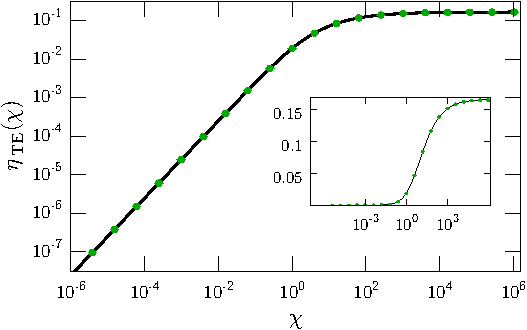
\includegraphics[width=0.8\textwidth]{fig/temp/eff_TE_atom_wall}
  \caption[Planar Casimir--Polder TE energy as function of $\chi$]
  {Planar Casimir--Polder TE energy normalized to atom-conductor Casimir--Polder energy, plotted as a function of susceptibility $\chi$.  
    The calculations used $10^8$ paths, with $10^4$ points per path.
    The results for each $\chi$ were computed using the same ensemble of paths.
    The solid black line is the analytical result~(\ref{eq:etaTE}), and the points are the numerical
    values computed using Eq.~(\ref{eq:TE_CP_num}).  
    All values of $\chi$ were computed 
    using the same ensemble of paths.
    (The inset shows same data on a linear vertical scale.)
    }
  \label{fig:eff_TE_atom_wall}
\end{figure}

% Each path was generated with the v-loop algorithm~(\ref{eq:vloop}). 
% A single path time $\cT$ was sampled for each path by sampling from Eq.~\ref{eq:Tpower_law}, 
% where $\cT_0$ is the smallest path time that the part starting at $x_0$ would contact a planar surface a distance $d$ 
% away.  For TE integrands, a whole range of $\chi$ can be evaluated in parallel for a single path since 
% $\langle \epsr\rangle = 1+\chi\langle\Theta(x-d)\rangle$.  The path averaged occupation time can be computed once for a 
% given path, and re-used to compute the Casimir--Polder energy for various $\chi$.  

% The numerically sampled values agree well with the analytical result for the 
% efficiency $\eta(\chi)$.  The efficiency is the ratio of the TE Casimir--Polder energy between an atom and a dielectric 
% to the total Casimir--Polder energy for an atom and a perfectly conducting plate.  This approaches $1/6$ in the 
% strong-coupling limit---the remainder of the Casimir--Polder energy is provided by the TM polarization, which
% will be discussed further in Sec.~\ref{sec:TM_numerics}.

\begin{figure}
  \centering
  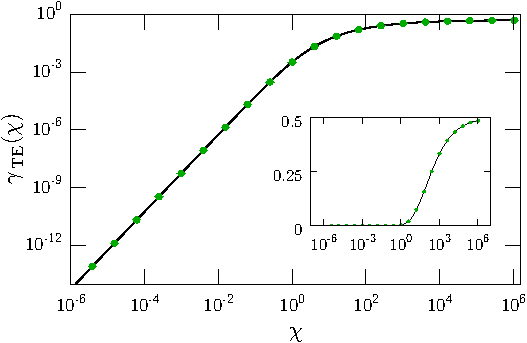
\includegraphics[width=0.8\textwidth]{fig/temp/eff_TE_2wall}
  \caption[Planar TE Casimir energy as function of $\chi$.]{
    Numerically calculated TE Casimir energy for two planes, normalized to Casimir energy between perfect-conducting plates,
    plotted as function of $\chi$.
    The black line shows the integral solution~(\ref{eq:gammaTE}), and the points show the numerical
    estimates computed using Eq.~(\ref{eq:TE_Casimir_num}).
    The calculations used $10^8$ paths, with $10^4$ points per path.  All values of $\chi$ were computed 
    using the same ensemble of paths.
    (Inset shows same data on a linear vertical scale.)}
  \label{fig:eff_TE_2wall}
\end{figure}

Figure~\ref{fig:eff_TE_2wall} shows the numerically computed Casimir energy between two planar dielectric interfaces
a distance $d$ apart, with dielectric function $\epsr(x) = 1+\chi\Theta(-x+d/2)+\chi\Theta(x-d/2)$.  
This is computed numerically by evaluating
\begin{align}
  E\supTE\subCP-E_0 
  &=-\frac{\hbar c\alpha_0}{8\pi^2}\biggdlangle  \frac{1}{2\cT_0^{2}P_x(x_0)}
  \bigg(1+\frac{1}{\langle\epsrab(x_k)\rangle^{3/2}}\nonumber\\
    &\hspace{5cm}-\frac{1}{\langle\epsra(x_k)\rangle^{3/2}}-\frac{1}{\langle\epsrb(x_k)\rangle^{3/2}}\bigg) 
\biggdrangle_{x_k,\cT,x_0},\label{eq:TE_Casimir_num}
\end{align}
where the ensemble average now also includes the integral over the starting positions $x_0$.
The starting positions are sampled from Eq.~(\ref{eq:xPower_law}), with $d_0=d$, 
which is twice the size of the region between the interfaces.  The results are robust
as this threshold is varied.   
In this case, it is necessary to compute both $\langle \theta(x-d_2)\rangle$ and $\langle \theta(d_1-x)\rangle$.
%The dielectric path average and the renormalized worldline integrand can then be quickly computed for multiple $\chi$.
One upshot of Monte Carlo sampling of $x_0$ and $\cT$ is that this is \emph{much} faster than directly evaluating 
the position and path time integrals on a path-wise basis.  However, it does give a larger sample
variance.  In fact, evaluating the Casimir energy takes roughly the same amount of time as the Casimir--Polder energy.  

\subsubsection{Error Scaling with Path Length $N$}
\label{sec:TE_convergence}
Some interesting scaling behavior was found by examining the relative error of the numerical 
estimates.  
In this case the systematic error is due to the discretization of the path.
The path integral was derived under the assumption that $N\rightarrow\infty$, while the numerical
calculations use a discrete path with a finite $N$.  
There is an additional statistical error associated with the finite number of paths.   However, for $N_{\text{path}}$ paths,
this error scales as $N_{\text{path}}^{-1/2}$, as is typical for Monte Carlo sampling error.  This is what determines
the noise floor in Figures~\ref{fig:conv_atom} and \ref{fig:conv_wall}.

\begin{figure}
  \centering
  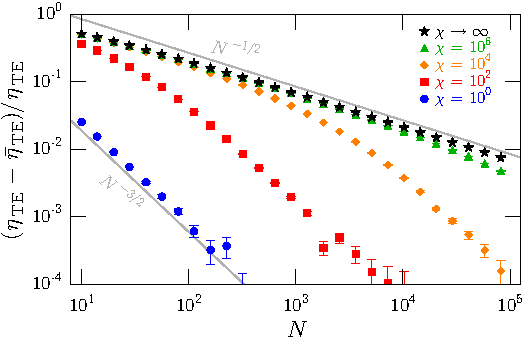
\includegraphics[width=0.8\textwidth]{fig/temp/conv_TEatomN3}
  \caption[Convergence of planar TE Casimir--Polder energy as function of $N$.  ]{
    Convergence of planar TE Casimir--Polder energy as a function of $N$.  
    Results plot the absolute relative error between the numerical estimates from Eq.~(\ref{eq:TE_CP_num})
    and the analytical result~(\ref{eq:etaTE}). 
    Different values of $\chi$ use the same ensemble of paths.
    Simulations used $10^8$ paths.}
  \label{fig:conv_atom}
\end{figure}

\begin{figure}
  \centering
  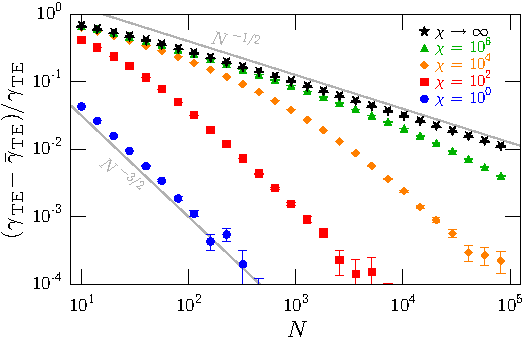
\includegraphics[width=0.8\textwidth]{fig/temp/conv_TE2wallN3}
  \caption[Convergence of planar TE Casimir energy as function of $N$ for various $\chi$.]{
    Convergence of planar TE Casimir energy as function of $N$.  Results plot the 
    absolute relative error between the numerical estimates from Eq.~(\ref{eq:TE_Casimir_num})
    and the analytical result~(\ref{eq:gammaTE}).
    Different values of $\chi$ use the same ensemble of paths.
    Calculations used $10^8$ paths, which sets the $10^{-4}$ noise floor.}
  \label{fig:conv_wall}
\end{figure}

As the path length $N$ increases for fixed $\chi$, the systematic error shows two different scaling behaviors.  
In the weak-coupling limit $\chi/N\ll 1$, the error scales as $N^{-3/2}$, while in the strong-coupling limit
$\chi/N\gg 1$, the error scales $N^{-1/2}$.  
These behaviours are analytzed in Ref.~\cite{Mackrory2016}, 
but we will summarize the basic reasoning here.  The numerical computations use discrete paths, 
while the path integral is only exact in the limit that $N$ is arbitrarily large.  The continuous paths considered by the path integral
have arbitrarily fine structure, and always have a non-zero probability to touch the dielectric body.
The discrete paths used in the numerical method miss those contributions, leading to a systematic error.  

In the weak-coupling limit $\chi/N\ll 1$, the numerical estimate is dominated by accurately estimating the sojourn
time $\langle\Theta\rangle$ for a given path.  Further increasing $N$ increases the accuracy of this 
estimate and the renormalized integrand.  The $N^{-3/2}$ scaling can be deduced by integrating the probability for a nonzero sojourn time
from each increment.  

In the strong-coupling limit $\chi/N\gg 1$, as soon as a path touches the surface the integrand immediately saturates
to its extreme value of negative one.
Thus the dominant error comes from underestimating the path time that this occurs.  The error 
is estimated by integrating the probability that a continuous path touched the surface
prior to the estimated first contact time.  This leads to a $N^{-1/2}$ scaling.

For a fixed $\chi$, the transition between both behaviors is observed at $N\sim\chi$. 
In the strict $\chi\rightarrow\infty$ Dirichlet limit, the numerical results and scaling 
arguments indicate that there will always be a $N^{-1/2}$ systematic error scaling in this case.   

\section{TM Casimir Numerics}
\label{sec:TM_numerics}

Numerically calculating Casimir energies due to the TM polarization is much harder than the TE case. 
This is due to the singular nature of the TM potential.
Even after regularization, and analytical path averaging, is still challenging to handle numerically.
We will develop a number of techniques to temper these difficulties.
As a side effect, they should have applications for more general Casimir worldlines.

The most daunting feature of the TM Casimir worldline~(\ref{eq:TM_Casimir}) is the singular TM potential~(\ref{eq:VsubTM}).
 A closed-form solution for the TM potential $V\subTM$ at a single planar boundary was found in Chapter~\ref{ch:feynman_kac}.
The ensemble-averaged solution for all Brownian paths between points $x_k$ and $x_{k+1}$ in time ${\Delta\cT}$ is 
\begin{align}
  v_{k,k+1}(x_k,x_{k+1})&:=\!  \Bigdlangle e^{-\int_0^{\Delta\cT} dt'\, V\subTM(x-d)}\Bigdrangle_{x_k\rightarrow x_{k+1}} \\
  %  =\,& \Theta[X_{k,k+1}]\big[1 + \sgn(d-x_k)e^{-2X_{k,k+1}/t}\tanh\Xi\big]
  % +\Theta[-X_{k,k+1}]\sech\Xi,
   \label{eq:TM_pot}
      &\,=\!\left\{\!\! \begin{array}{lc} 
          1  + \sgn(d\!-\!x_k)\tanh\Xi\, e^{-2(d-x_k)(d-x_{k+1})/{\Delta\cT}} &\!\! (d\!-\!x_k)(d\!-\!x_{k+1})\!>0\\
          \sech\Xi & \!\!(d\!-\!x_k)(d\!-\!x_{k+1})<0.
        \end{array}
        \right.  
\end{align}
This ensemble-averaged solution was plotted in Figure~\ref{fig:TMpot}, 
for $x_k$ and $x_{k+1}$ on either side of the interface at various values of $\Xi$.
The solution varies between zero and one for paths that start inside a dielectric body, or cross an vacuum-dielectric interface.
For paths starting in vacuum outside a dielectric body, the solution varies between one and two.  The extreme values of zero and 
two only appear in the strong-coupling limit close to the surface.

This solution can be used in the path integral by identifying averages of sub-paths
between discrete points with the analytical solutions.
The path averaged exponential potential can be refined into arbitrarily many steps between $\vect{x}_k$ and $\vect{x}_{k+1}$
at times $\cT_k$ and $\cT_{k+1}$.  Each exponential potential can be averaged over all possible continuous sub-paths
between $x_k$ and $x_{k+1}$, with the result,
\begin{align}
  \biggdlangle \frac{e^{-\cT\langle V\subTM\rangle}}{\langle\epsr\rangle^{1/2}}\biggdrangle \approx &
  \biggdlangle \frac{1}{\langle \epsr\rangle^{1/2}}\prod_{k=1}^N
  \bigglinklangle \exp\left(-\int_{\cT_k}^{\cT_{k+1}} dt\, V\subTM[x(t)]\right)\bigglinkrangle_{x_k\rightarrow x_{k+1}}
    \biggdrangle\\
 =& \biggdlangle \frac{1}{\langle \epsr\rangle^{1/2}}\prod_{k=1}^N  v_{k,k+1}    \biggdrangle,
  \end{align}
  where $\linklangle\cdots\linkrangle$ denotes an average over continuous sub-paths between $x_k$ and $x_{k+1}$.
%   It is not strictly necessary to include the dielectric average in the averaging over
% sub-paths, since the dielectric average is a much smoother function that varies more slowly.  % Taking the dielectric into the average of sub-paths would lead to 
% even better results, but those analytical solutions are difficult to calculate.
% The integrand can be built up even for a discrete Brownian bridge of length $N$, 
% by multiplying the appropriate TM potential terms~(\ref{eq:TM_pot}) along the path, and then dividing
% by the path average of the dielectric $\langle\epsr\rangle$.  

% This notion of replacing a singular potential with its ensemble averaged value between two end points
% is a powerful one.  This technique also offers an improvement on the accuracy for Dirichlet boundary conditions,
% and which will be discussed further in Secs.~\ref{sec:general_gradient} and \ref{sec:accel_converge}.

\subsection{Scaling of the Averaged TM Potential with Path Length $N$}

The numerical properties of the solution can be examined by considering a simplified path integral
that only includes a single TM potential a distance $d$ away,
\begin{align}
  I=\dlangle e^{-\int_0^\cT dt\,\VTM[x(t)]}\drangle_{\vect{x}(t)}
=\,& \Biggdlangle \prod_{k=0}^{N-1}
  \bigglinklangle  e^{-\int_0^{\Delta \cT} dt\,\VTM[x(t)]}\bigglinkrangle_{x_k\rightarrow x_{k+1}}\Biggdrangle_{\vect{x}_k}\\
=\,&\Biggdlangle \prod_{k=0}^{N-1}
  v_{k,k+1}\Biggdrangle_{\vect{x}_k}.
  \label{eq:Vsimp}
\end{align}
The left-hand ensemble average is over continuous Brownian bridges, whereas the second ensemble
average runs over discrete Brownian bridges (and averaging over continuous sub-paths between points on the 
discrete path, as indicated by $\linklangle\cdots\linkrangle$).
In this case, the exact value of the integral is just the TM potential solution Eq.~(\ref{eq:TM_pot}),
for $x_k,x_{k+1}\rightarrow x_0$.  The right hand side can be computed numerically to examine its scaling with $N$.

Figure~\ref{fig:TM_histogram} shows a histogram of numerically estimated values for closed Brownian paths 
interacting with the TM potential.  Each Brownian path is generated via the v-loop algorithm~(\ref{eq:unit_vloop}),
and scaled by $\sqrt{\cT}$.  The total contribution from each path is the product of the TM solutions~(\ref{eq:TM_pot}) for every
step along the path.
The direct estimate of the TM potential shows a wide spread of values over different paths.
 Most paths return values close to zero, while a few rare paths return very large values.  
This suggests that the plain Gaussian paths 
are poorly suited to this problem, and that the path generation scheme should be modified.
Given a large enough ensemble, this method eventually converges to the right answer, but it displays
unacceptably large statistical errors.  

\begin{figure}
  \centering
  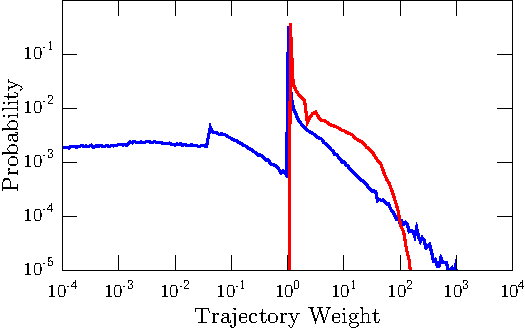
\includegraphics[width=0.8\textwidth]{fig/numerics/TM_normhist}
  \caption[Histogram of Accumulated Numerical TM Estimates]
  {Histogram of accumulated numerical TM estimates, for Gaussian (blue) and birth-death Gaussian (red).
    Calculations used $10^6$ paths, with $N=200$ points per path, $\chi=100$, $d=1$, and $\cT=1.$
    The correct value for the integral at these parameters is $(I=1.595)$.  The Gaussian estimate is $(1.40\pm 0.14)$.
    The birth-death estimate is $(1.602\pm 0.006)$.
    (The birth-death method is discussed in Sec.~\ref{sec:birth_death}.)
    The Gaussian distribution extends off to zero, 
    while the birth-death distribution has truncated peak at zero.}
\label{fig:TM_histogram}
\end{figure}

\subsubsection{``TM-Gaussian'' Paths}

\begin{figure}
  \centering
  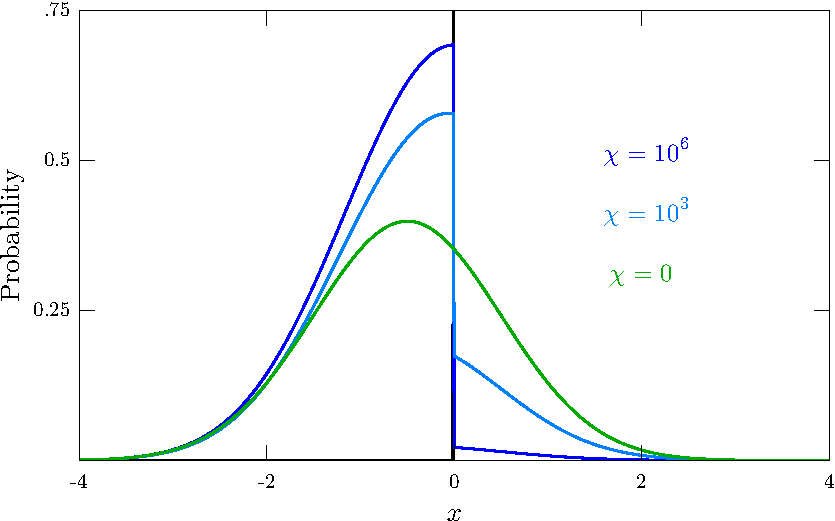
\includegraphics[width=0.8\textwidth]{fig/numerics/probTM}
  \caption[Combined TM-Gaussian probability distribution.]{
    Combined TM-Gaussian probability distribution plotted for various $\chi$.  Corresponds
    to a single term in the product in Eq.~(\ref{eq:TMGaussian_joint}).
    Increment starting position is $x=-1$, and $\cT=1$.  The boundary is at the origin. }
\end{figure}

One possible solution to the fluctuations is to sample from a combination of a Gaussian
and the path-averaged exponential~(\ref{eq:TM_pot}) for the path increment.  Since the 
path-averaged exponential is taken into account in the sampling, more representative values should 
be chosen, which should reduce the number of extreme values of the estimates.
In this case, the total probability distribution for the paths is 
\begin{align}
  P(x_1,\ldots ,x_{N-1}) = \prod_{k=0}^{N-1}\frac{e^{-(x_{k+1}-x_k)^2/(2\Delta\cT)}}{\sqrt{2\pi\Delta\cT}}
  \bigglinklangle e^{-\int_0^{\Delta \cT}dt\, \VTM}\bigglinkrangle_{x_k\rightarrow x_{k+1}}.\label{eq:TMGaussian_joint}
\end{align}
In the same manner as the v-loops, the Gaussian probability distribution can be decoupled into a
set of random variables, where from Eq.~(\ref{eq:open_vloop}), the argument of each of those Gaussians 
involves ${z_k = (x_k-c_{k}x_{k-1})/\sqrt{c_k\Delta \cT}}$.
After implementing the v-loop change of variables, 
the probability distribution~(\ref{eq:TMGaussian_joint}) can be written as
\begin{align}
  P(x_1,\ldots ,x_{N-1}) = v_{N,N-1}\prod_{k=0}^{N-1}\cN_{k+1}P\supTM_{k+1}(x_{k+1}),
\end{align}
where the new probability distribution for $x_{k+1}$ is 
\begin{align}
  P\supTM_{k+1}(x_{k+1}):=\cN^{-1}_{k+1}\frac{e^{-(x_{k+1}-c_k x_k)^2/(2c_k\Delta\cT)}}{\sqrt{2\pi c_k\Delta\cT}}v_{k,k+1}(x_k,x_{k+1}),
  \end{align}
with normalization constant 
\begin{align}
  \cN_k=\int dy\, \frac{e^{-(y-c_k x_k)^2/(2c_k\Delta\cT)}}{\sqrt{2\pi c_k\Delta\cT}}v_{k,k+1}(x_k,y).
\end{align}
The crucial point is that the $P\supTM_{k+1}$ can act as the probability distribution for $x_{k+1}$, accounting only for the present position $x_k$. 
Although the present position $x_k$ is still coupled to future positions via $v_{k+1,k+2}$, the sampling procedure ignores
that and samples $x_{k+1}$ based solely on $P\supTM_{k+1}$.  
The probability distribution can be put into a convenient numerical form by completing the square to account
for $v_{k,k+1}$.  The resulting piecewise Gaussian probability distributions can be split 
into ``no-crossing'' and  ``crossing'' terms, where
\begin{align}
  P\supTM_{k+1}(x_{k+1})
  = \cN_{k+1}\big\{& \Theta[(d-x_k)(d-x_{k+1})]P\supTM_{\text{NC},k+1}(x_{k+1})\nonumber\\
  &+  \Theta[-(d-x_k)(d-x_{k+1})]P\supTM_{\text{C},k+1}(x_{k+1})\big\}
\label{eq:PTM_k}
\end{align}
and
\begin{align}
P\supTM_{\text{NC},k+1}(x_{k+1})&=  \sgn(d-x_k)\dfrac{\tanh\Xi}{\sqrt{2\pi c_k \Delta\cT}} e^{-2(1-c_k)d(d-x_k)/\Delta\cT} e^{-(x_{k+1}-c_k(2d-x_k))^2/(2c_k \Delta\cT)}\nonumber\\
&  \hspace{0.5cm}+ \dfrac{e^{-(x_{k+1}-c_k x_k)^2/(2c_k \Delta\cT)}}{\sqrt{2\pi c_k \Delta\cT}}  \\
P\supTM_{\text{C},k+1}(x_{k+1}) &=\dfrac{\sech \Xi}{\sqrt{2\pi c_k \Delta\cT}}e^{-(x_{k+1}-c_k x_k)^2/(2c_k \Delta\cT)}.
\end{align}
The normalization constant can be evaluated in two parts, $\cN_{k+1}=\cN_{k+1}^{\text{C}}+\cN_{k+1}^{\text{NC}}$, 
 with the result
\begin{align}
  \cN_{k+1}^{\text{C}}=\,& \frac{1}{2}\left[1+\sgn(d-x_k)\, \erf\!\left(\frac{d-c_k x_k}{\sqrt{2 c_k \Delta\cT}}\right)\right] \nonumber\\
  &+\sgn(d-x_k) \frac{\tanh\Xi}{2}\left[1+ \sgn(d-x_k)\,\erf\!\left(\frac{d(1-2c_k)+ c_kx_k}{\sqrt{2c_k \Delta\cT}}\right)\right]\nonumber\\
  & \hspace{2cm}\times e^{-2(1-c_k)d(d-x_k)/\Delta\cT} \\
 %  &=\frac{1}{2}\left[1- \erf\left(\frac{d-c_k x_k}{\sqrt{2 c_k \Delta\cT}}\right)\right]
 % - \frac{\tanh\Xi}{2}\left[1- \erf\left(\frac{d(1-2c_k)+ c_kx_k}{\sqrt{2c_k \Delta\cT}}\right)\right]e^{-\frac{2(1-c_k)d(d-x_k)}{\Delta\cT}}\text{d<x_k}.
% \end{align}
% \begin{align}
\cN_{k+1}^{\text{NC}}=\,& \frac{\sech\Xi}{2}\left[1-\sgn(d-x_k) \erf\left(\frac{d-c_k x_k}{\sqrt{2 c_k \Delta\cT}}\right)\right].
\end{align}
The probability distribution~(\ref{eq:PTM_k}) can be sampled via the following procedure.
First, note that the probability distributions involve truncated Gaussians in $x_{k+1}$.  The truncation
occurs at the surface $x_{k+1}=d$, since the probability distribution was split based on whether path increments cross
through the surface or not.
At each step the simulation picks the crossing or no-crossing branch of the probability distribution
cased on the relative weights of $\cN_{k+1}^\text{C}$ and $\cN_{k+1}^\text{NC}$, picking the crossing branch 
if $\cN_{k+1}^{\text{C}}/\cN_{k+1}<u$ where $u$ is a uniform random number.  
If the crossing branch is chosen, then a deviate is sampled from the truncated Gaussian distribution.
Otherwise, if the no-crossing branch is chosen, then depending on the sign of $\sgn(d-x_{k+1})$, there are another two options.
If $\sgn(d-x_{k+1})>1$, then one of the Gaussians is picked based on their relative probability of occurring,
and a deviate is sampled from one of them.
If however, $\sgn(d-x_{k+1})<1,$ then the rejection method is used to generate a deviate.
In the rejection method, a deviate is sampled from a ``proposal'' distribution $P_1(x)$(such as one of the Gaussians),
and accepted with a probability $P_2(x)/P_1(x)$, where  $P_2$ is the target distribution~\cite{NumRecipe}.
In the other cases, the truncated Gaussian distributions can be sampled quickly via the inverse error function.  

While this method does improve performance, it still relies on taking a product of $N-1$ normalization factors $\cN_{k+1}$,
where $0<\cN_{k+1}<2$.  This leads to the same problems with large statistical errrors as the plain Gaussians
as the path length $N$ is increased.  It is also much more involved to implement than the plain Gaussian
approach.

\subsubsection{Birth-Death Path Swarm}
\label{sec:birth_death}
Both the plain Gaussian and TM-Gaussian paths can be rescued by further adjusting the sampling procedure.
In both cases, the path can accumulate a large weight.  After $k$ steps,
the weight is $w_k=\prod_{j=1}^k\nu_j$, where $\nu_j$ represents either $v_{j,j+1}$ for Gaussian paths or $\cN_j$
for TM-Gaussian paths.  Most paths propagating close to the surface will acquire 
a number of large weights with $\nu_j>1$ when they are on the vacuum side of the interface, 
and small weights $0<\nu_j<1$ when they are on the dielectric side of the interface.  
The logarithm of the accumulated weight is $\log w_k = \sum_{j=1}^k\log \nu_j$.  
Since the $\nu_j$ are random variables (both $v_{k,k+1}$ and $\cN_k$ are functions of an underlying random path),
then from the central limit theorem, we would expect $\log w_k$ to be normally distributed, with some standard deviation $\sigma^2$. 
(The central limit theorem applies to the sum of a large number of independent random variables---it maybe 
that the independence assumption is violated in this case, as the path position acts as a memory.)
Nevertheless, this predicts that the accumulated weight is expected to behave as a log-normal deviate, with variance ${e^{\sigma^2}(e^{\sigma^2}-1)}$.    
Since $\sigma^2$ grows linearly with $N$, the variance of the product $w_k$ would grow exponentially with $N$.  
Note that the mean would still have the correct value, but the variance, and thus sampling error would
grow unacceptably as $N$ increases.

% A large number of paths will yield very low values, and a lot of computer time would be wasted on simulations
% which computing numbers very close to zero.  A few rare paths would skirt outside the surface, accumulating
% very large weights, and contributing a lot to the Casimir energy.  Together these lead to large statistical
% fluctuations, which make it hard to get sufficient averaging for even moderately fine paths $N\sim 100$.
% Note that both types of paths will contribute to the Casimir energy.

The path generation for either method can be modified as follows.  The weight $w_k$ is effectively treated as 
the fitness function for the path.  Paths with large weights will spawn further paths (``birth''), while paths with
small weights will be terminated and return zero (``death'').  At each step of the path, the 
accumulated weight must be checked.
If the weight is becoming small, $w_k<0.5$ then the weight should be compared with a uniform random number $u$.
If $w_k<u$, then the path dies; alternatively, if $w_k>u$, then 
the path survives and the weight is reset $w_k=1$.  That is the death process.
In an ensemble average, an average fraction of the paths $u$ survive the death process, which gives 
the correct average value.
If the weight becomes large, $w_k>2$, then divide the weight in two, and assign each half to 
two independent paths.
Altogether, this is called a ``birth-death'' process, and should be applied at every step of the random path.
If a path survives for $N$ steps, then its contribution is added to a running total for this swarm.
Once all of the paths have either died, or reached the end, the accumulated total for this swarm is then
renormalized (by subtracting 1), and added to the running totals used to estimate the mean and variance.  
Implementing the deaths ensures that the number of computations  does not grow exponentially as a function 
of path length, while the birth process ensures that successful trajectories with a large weight have 
contribute more to the path integral.  The death process speeds up the computation by not computing 
negligible corrections to the swarm value.  

The birth-death process is a very simple Markov Chain Monte Carlo method.  The birth-death
process modifies the preferred motions based on the accumulated weight.  Paths are likely to be born
on the vacuum side of interfaces, and they are likely to die on the dielectric side of the interface.
Far away from the interface on either side, the paths are unlikely to branch or terminate.  

Similar terms are discussed throughout stochastic processes literature.
As a matter of nomenclature, it is worth distinguishing the birth-death process we are 
using from the more popular birth-death process used in queuing theory.  In queuing theory, 
the number of objects in a queue randomly increases and decreases at a fixed average rate.
In our case, that rate depends on the past behavior of the system, and where it has gone.  
The process used here is closer to the genealogical methods for evaluating path integrals discussed by Del Moral~\cite{DelMoral2004}.
A similar genealogical idea has been used in quantum trajectory simulations~\cite{Jacobs2010a}, which is a
technique for simulating open quantum systems.  In that variant, each quantum state in an ensemble carries 
a probability weight.  If that weight becomes too small, then that random trajectory is discarded,
and another more successful trajectory is split in two, and given half the weight.   
A similar method has been used to discuss simulating rare events, such as the extreme tails of a Gaussian.
In that case, one splits trajectories based on whether they exceed a certain threshold criterion~\cite{Glasserman1999,Garvels2000}.
These methods essentially reward the trajectories or paths of the system that enter regions with a large
contribution to the integral (or other figure of merit).  Thus more computational effort is spent in 
regions with significant contributions to the result.  

\begin{figure}
  \centering
  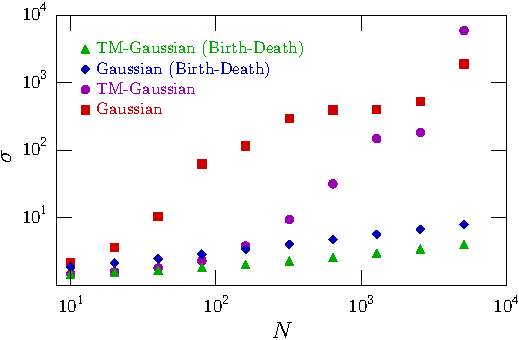
\includegraphics[width=0.8\textwidth]{fig/numerics/TM_scalingN}
  \caption[Scaling of standard deviation for estimated TM potential as function of $N$ for four methods.]
  {Scaling of standard deviation for estimated TM potential as function of $N$ for four methods.  
    Eq.~(\ref{eq:Vsimp}) is evaluated for both Gaussian increments, TM-Gaussian increments, 
    and then for birth-death variants of both methods.  
  All combinations of Gaussian paths increments and combined TM-Gaussian steps, with raw values and 
  birth-death.}
\label{fig:TM_scalingN}
\end{figure}

Figure~\ref{fig:TM_scalingN} shows how the Gaussian and TM-Gaussians estimates of the simple path integral
scale with the path resolution.  The birth-death process has been applied to both ways of generating paths.
The birth-death process reduces the variance, and makes both methods much more tractable.
The difference between Gaussian and TM-Gaussians is small under the birth-death process.
Given that small difference, and the relative simplicity of the Gaussians, we have opted to 
use the birth-death process in conjunction with Gaussians throughout the remainder. 

\subsection{Monte Carlo Sampling for the Path-Time}

\label{sec:expT-sampling}
When using the birth-death method for generating paths, the TM polarization requires a 
slightly different sampling method for generating path times $\cT$.  
In some limited cases it may be possible to estimate a minimum $\cT_0$ where 
the integrand is small for a given path, and a path is unlikely to have branched or birthed new paths.  
For paths starting on the vacuum side near a dielectric, the accumulated
potential at small path times is approximately ${\prod_k( 1+\tanh\Xi e^{-2(d-x_k)(d-x_{k+1})/\Delta\cT})}$,  
which turns on smoothly in $\cT$.
In that case, $\cT_0$ can be estimated from the time an initial, fiducial path would contact a surface and the 
integrand would turn on.  The path time can be sampled from the power law distribution~(\ref{eq:Tpower_law}).
The birth-death process then proceeds starting with a version of the initial path that is scaled by $\sqrt{\cT}$.  

However, in a two-body geometry that sort of estimation fails.
The renormalized integrand is only nonzero for paths that come close to both surfaces.
Since the birth-death method may split the trajectory, it is not always possible to reliably
find a minimum time $\cT_0$ when the renormalized integrand turns on.  (A very small $\cT_0$ could be picked, 
where the path has no chance of touching the surface, but most computations would return zero,
 since the most probable $\cT$ are close to $\cT_0$.)
As a result, it is not possible to estimate for a single trajectory a lower bound $\cT_0$ 
for which the path does not branch, but is also close to when the integrand turns on.  

Since the birth-death method essentially enlarges the ensemble of paths selected, its turn on
mimics the probability for a Brownian bridge to touch a surface.
The probability for a Brownian bridge to touch a surface a distance $d$ away in path time $\cT$ is 
\begin{equation}
  P_{\text{touch}}(\cT) = e^{-2d^2/\cT}.
\end{equation} 
The combined potential term ${\prod_kv_{k,k+1}}$,  also has a similar dependence.  
This could be combined with the $\cT^{-(1+D/2)}$ power law for a new probability distribution.  
\begin{equation}
  P_{\text{exp-T}}(\cT;\cT_0,s) = \frac{\cT_0^{s-1}}{\Gamma[s-1] \cT^s}e^{-\cT_0/\cT}\label{eq:expT},
\end{equation}
where $s>1$ and $\cT_0>0$.  
%  The exponential factor effectively models the finite touching 
% probability for Brownian bridges starting at the origin to touch a planar surface a distance $d$ 
% away in time $\cT$, $P_\text{touch}=e^{-2d^2/\cT}$. 
The probability distribution~(\ref{eq:expT}) can be transformed to $u=\cT_0/\cT$, for 
which the probability distribution is
\begin{equation}
  P_{\text{exp}-1/\cT}(u;s) = \frac{u^{s-2}}{\Gamma[s-1]}e^{-u}.
\end{equation}
% where we had to include $du/d\cT= -(\cT_0)/\cT^2=-1/(\cT_0u^2)$ for the change
% of measure.  
The new variable $u=\cT_0/\cT$ has the form of a gamma distribution, which has probability density 
\begin{equation}
  f(x) = \frac{x^{a-1} e^{-x/b}}{\Gamma(a)b^a}.  
\end{equation}
where $a>0$ and $b>0$ are the shape and scale parameters respectively~\cite{Devroye2003}.  
For small integer or half-integer powers $a$, there are some simple methods for generating 
gamma deviates $g_i$.  
A sum of gamma deviates $=\sum_{i=1}g_i$ with shape parameters $a_i$, is also a gamma deviate
with shape parameter $\sum a_i$~(see pg. 402 of Devroye~\cite{Devroye2003}).  
A gamma deviate with shape parameter $a=1$ is an exponential deviate, $e_i=-\log(u)$ where 
$u$ is a uniform random number.  
In particular, this means the sum of $n$ exponential deviates yields a gamma 
deviate with shape parameter $a=n$.  
In addition, if $z$ is a standard normal variable, then $z^2/2$ is gamma distributed with $a=1/2$.
For small integer powers, $\cT$ is distributed according to
\begin{equation}
  \cT\sim \frac{\cT_0}{-\sum_{i=1}^{s}\log u_i},
\end{equation}
while for half-integer powers, 
\begin{equation}
  \cT\sim \frac{\cT_0}{-\sum_{i=1}^{\text{floor}(s)}\log u_i+z^2/2}.
\end{equation}
The integer powers are useful for estimating zero temperature Casimir energies. The half-integer powers
naturally emerge when considering the thermal Casimir energy, or derivatives of the Casimir energy 
such as the force.  
This distribution can also be used to sample times $\cT$
even for TE integrands.  In that case however, it is possible the generated path will not
touch all bodies and merely return zero, which will increase the variance of the numerical
estimated energy.  

\subsection{Gradient Estimation}

Computing the TM Casimir--Polder energy~\ref{eq:TM_Casimir_Polder}, requires taking two spatial derivatives
of the worldline path integral.
Furthermore, in some experiments on the Casimir--Polder effect such as BEC experiments~\cite{Harber2005}, 
the Casimir--Polder potential is estimated from how it shifts the frequency of the atom's oscillations
in a harmonic potential.  This frequency shift is calculated by taking two derivatives of the Casimir--Polder
potential.   For the TM polarization within the worldline method, this would require four spatial 
derivatives, so it is essential to be able to efficiently compute these derivatives for worldline path integrals.  

Consider a generic worldline path integral involving pinned Brownian motions in path time $\cT$ with starting point $\vect{x}_0$
\begin{equation}
  I(x_0)=\dlangle \Phi(x_0,x_1,\ldots,x_{N-1})\drangle_{\vect{x}(t),\vect{x}(0)=\x0}.
\end{equation}
The function $\Phi$ depends on the whole path, and serves as a placeholder for the path averaged dielectric
or TM potentials.  The $n^\text{th}$ derivative of this path integral with respect to the starting
position is 
\begin{equation}
  \partial_0^nI(x_0)=\frac{\partial^n}{\partial x_0^n}\dlangle \Phi\drangle_{\vect{x}(t),\vect{x}(0)=\x0}.
\end{equation}
We will discuss how to evaluate this derivative with both the finite difference method 
and the partial-averaging approach.

\subsubsection{Finite Differences}
\label{sec:finite_difference}
The finite difference method is simplest method for numerically evaluating derivatives.
 It has the great virtue of simplicity, since it only requires that we evaluate the function multiple times.  
For smooth functions, the finite difference method works well, but it behaves poorly when applied to
stochastic, discontinuous functions such as the worldline path integral. 

For example, consider the first derivative of the TE Casimir--Polder worldline integrand,
at a dielectric step $\epsr=1+\chi\Theta(x-d)$.  The finite difference integrand is
\begin{equation}
  \partial_0\Bigdlangle \,\langle\epsr[\vect{x}(t)\rangle^{-3/2}-1\Bigdrangle_{\vect{B}_k}
  \!=\! \frac{1}{\Delta s}\Bigdlangle \, \langle\epsr[\vect{x}_0+\Delta s\hat{r}_i+\sqrt{\cT}B_k]\rangle^{-3/2}
  -\langle\epsr[\vect{x}_0+\sqrt{\cT}B_k]\rangle^{-3/2}\,\Bigdrangle_{\vect{B}_k},
\end{equation}
where $\Delta s$ is the finite difference step size, $\vect{B}_k$ is a closed unit Brownian bridge, 
and $\hat{r}_i$ is a Cartesian unit vector.
This can be evaluated on a path-wise basis.  
In order to be accurate, the step size $\Delta s$ must be small, since the error in this approximation 
to the derivative is $\order[(\Delta s)^2]$.
Unfortunately, that limit leads to large fluctuations.
If the finite difference is much smaller than a typical path increment, $\Delta s\ll \sqrt{\Delta\cT}$, 
the estimates for path averaged dielectric $\langle\epsr(\vect{x}_0)\rangle$ for the two starting positions
are likely to be the same, so the estimate is zero.  
In rare circumstances, a point is within $\Delta s$ of the surface, and the finite difference returns
the large value of $(\Delta s)^{-1}$.
Thus most paths estimate zero derivative, but a few paths return a large answer.  This leads to 
growing fluctuations.  This problem is even worse for higher derivatives.  
%In evaluating the finite difference it is best to use the same random numbers to generate the path~\cite{Asmussen2008,Glasserman2004}.

The finite difference method is also problematic for the birth-death method for TM potentials.  
In that case, as the starting position of the paths varies, a different family
of birth-death paths may be generated, which further compounds the fluctuation problem.    

\subsubsection{Malliavin Calculus}
Similar derivatives are required in quantitative finance, where the sensitivity of a financial 
product to variations its underlying parameters must be estimated~\cite{Glasserman2004}.  This could be done via a finite
difference method, but that behaves poorly.  
Since financial simulations also typically involved averages over simulated Brownian motions, similar problems emerge.
One promising approach for worldline applications is based on the Malliavin calculus, which 
is formally discussed in Ref.~\cite{Nualart2006, Malliavin2006, DiNunno2009}.
Less formal (and more understandable) discussions of the Malliavin approach are presented in Refs.~\cite{Chen2007,Kohatsu-Higa2003}.
In the Malliavin approach, the derivative can be estimated by multiplying the integrand by
a suitably chosen weight function, which depends on the nature of the derivative and the random path.
The Malliavin calculus is essentially functional differentiation with respect to the Brownian motion, 
and an associated integration by parts formula.   
The Malliavin weights can be derived by exchanging derivatives with respect to a parameter for
derivatives with respect to the Brownian motion, and integrating by parts~\cite{Kohatsu-Higa2004}.  
The Malliavin results can also be recovered via the likelihood-ratio method\footnote{
In the likelihood ratio method~\cite{Broadie1996}, a derivative with respect to a parameter $\theta$ of a stochastic average is evaluated 
as $\partial_\theta\dlangle \Phi(x)\drangle = \int dx\,\Phi(x)\partial_\theta P(x,\theta) 
= \dlangle \Phi(x)\partial_\theta\log P(x,\theta)\drangle$,
where $\partial_\theta\log P$ is the likelihood function.  
The original sampling method can be used to evaluate this derivative, so $\dlangle\Phi\drangle$ and its derivatives
$\partial_\theta\dlangle \Phi\drangle$ can be evaluated using the same random samples.}
in conjunction with partial-averaging along the Brownian motion~\cite{Chen2007}. 
In either case, one replaces differentiation for
evaluating a reweighted function, where the form of the function depends on the required derivatives.
The advantage is the same sample paths can be used for both the estimate and its derivative.  
While the Malliavin approach to derivative estimation did not yield better results for the worldline
method, it did inspire a similar approach, with similar virtues.   

\subsubsection{Partial Averaging Gaussian Paths}

\label{sec:partial_averaging}
Let us consider directly evaluating the derivative on the generic path integral
\begin{align}
  \partial_0^nI(x_0)&=\frac{\partial^n}{\partial x_0^n}\int \prod_{j=1}^{N}dx_j\delta(x_N-x_0)
  \prod_{k=1}^{N}\frac{e^{-(x_{k+1}-x_k)^2/(2\Delta\cT)}}{\sqrt{2\pi\Delta \cT}}\Phi(x_0,x_1,\ldots x_{N-1}).
\end{align}
Note there is some freedom here, which leads to slightly different approaches.  
If the integration variables are shifted to $y_k=x_k-x_0$, then the derivatives only act on $\Phi$.
This is close to the approach used in the finite difference approach where the whole path was translated by
$\Delta s$.  
If however, the variables are unchanged, and the derivatives are evaluated, the derivatives
act on the coupled Gaussian.
\begin{align}
  \partial_0^nI(x_0)&=\int \prod_{j=1}^{N-1}dx_j
  \frac{\partial^n}{\partial x_0^n}\prod_{k=0}^{N-1}\frac{e^{-(x_{k+1}-x_k)^2/(2\Delta\cT)}}{\sqrt{2\pi\Delta \cT}}\Phi(x_1,\ldots x_{N-1}).
\end{align}
The derivatives acting on $\Phi$ have been neglected, which effectively assumes that 
$\Phi$ does not vary significantly at the path origin.  
The derivatives of the Gaussians yield Hermite Polynomials, which are defined via
\begin{equation}
  \frac{d^n}{dx^n} e^{-(x-\mu)^2/a^2} = (-a)^{-n} H_n\bigg(\frac{x-\mu}{a}\bigg)e^{-(x-\mu)^2/a^2}.
\end{equation}
The Gaussians for the first and last steps can be differentiated $n$ times with respect to $x_0$,
with the result
\begin{align}
&\partial_0^n\frac{1}{2\pi \Delta\cT^2}e^{-(x_0-x_1)^2/(2\Delta\cT)-(x_0-x_2)^2/(2\Delta\cT)}\nonumber\\
&=\frac{1}{\sqrt{\pi\Delta\cT}\sqrt{4\pi\Delta\cT}} 
\left(\frac{-1}{\sqrt{\Delta\cT}}\right)^n H_n\left(\frac{x_0-\bar{x}_1}{\sqrt{\Delta\cT}} \right)
\exp\left[-\frac{(x_0-\bar{x}_1)^2}{\Delta\cT} - \frac{(\Delta x_1)^2}{4\Delta\cT}\right],\label{eq:Hermite_init}
\end{align}
where the following have been defined
\begin{equation}
\Delta x_k:=x_{N-k}-x_k \qquad \bar{x}_k:=(x_k+x_{N-k})/2,
\end{equation}
and used with $k=1$.
The differentiated path integral is then
\begin{align}
  \partial_0^nI(x_0)&=\biggdlangle
  \left(\frac{-1}{\sqrt{\Delta\cT}}\right)^n H_n\left(\frac{x_0-\bar{x}_1}{\sqrt{\Delta\cT}}\right)
 \Phi(x_1,\ldots x_{N-1})
\biggdrangle_{x_k},
\end{align}
where the Gaussians have been restored to their usual form and the path integral has been rewritten in ensemble average form.
In principle this method would also work for estimating the derivatives.  However as written, this 
will have large numerical fluctuations.  In particular, the answers will be distributed around zero, with
with some reweighting due to $\Phi$, which preferentially weights certain values.  However, the overall answer scales
as $(\Delta\cT)^{-n/2}$.  As the path length $N$ increases, the fluctuations will scale
as $N^{n/2}$ which is unacceptable.    

\begin{figure}
  \centering
  \includegraphics[width=0.4\linewidth]{fig/int-by-parts}
  \caption[Partial averaging along a path]{Partial averaging along a path close to a surface.  The extent 
    of the averaging is chosen that $x_m$ and $x_{N-m}$ are as large as possible, while being unlikely to enter the dielectric.}
  \label{fig:int-by-parts}
\end{figure}

This method can be improved by partial averaging over the path.
In particular, we assume that $\Phi=\prod_{k=1}^N\phi(x_k)$, 
and each $\phi(x_k)$ only varies significantly for $x_k\sim d$, and when $x_k\ll d$, $\phi(x_k)$ can otherwise
be approximated as a constant.  An example of this geometry is illustrated in Figure~\ref{fig:int-by-parts}, 
for an atom near a dielectric surface.  
For the first and last $m$ points along the path, the integrals can be carried out assuming that $\Phi$ is 
approximately constant.  
The result for integrating out $x_1,\ldots,x_{m-1}$ and $x_{N-m+1},\ldots,x_{N-1}$ in Eq.~(\ref{eq:Hermite_init}) is
\begin{align}
  \partial_0^nI(x_0)&=\int\prod_{k=m}^{N-m}dx_k\left(\frac{-1}{\sqrt{\Delta\cT}}\right)^n 
  H_n\left(\frac{x_0-\bar{x}_m}{\sqrt{m\Delta\cT}}\right)
  e^{-(x_0-\bar{x}_m)^2/\cT_m -(\Delta x_m^2)/4\cT_m}\nonumber\\
  &\times \prod_{k=m}^{N-m+1}
\frac{e^{-(x_{k+1}-x_k)^2/(2\Delta\cT)}}{\sqrt{2\pi\Delta \cT}}\Phi(x_1,\ldots x_{N-1}).\\
 &= \biggdlangle
  \left(\frac{-1}{\sqrt{m\Delta\cT}}\right)^n H_n\left(\frac{x_0-\bar{x}_m}{\sqrt{m\Delta\cT}}\right)
  \Phi(x_m,\ldots x_{N-m})\label{eq:partial_avg_grad}
  \biggdrangle.
\end{align}
% The composition rule for Hermite polynomials and Gaussians follows by first integrating out the intermediate coordinates, 
% and then differentiating the results.  
The combination of the Hermite polynomial is effectively the desired Malliavin weighting function.
This approach has replaced differentiation
with multiplication by a function that does not fluctuate more as the path length changes.
This method naturally generalizes to other Cartesian derivatives.  The path can be generated 
using the v-loop algorithm~(\ref{eq:unit_vloop}), and the relevant parts of the path can be 
used to evaluate Eq.~(\ref{eq:partial_avg_grad}).

Each integration over an intermediate coordinate makes some small error in approximating $\Phi$ as constant.  
The partial averaging should only be carried out to the point where that error can no longer be ignored.
If the function $\Phi$ starts to deviate from a constant at $x=d$, such as for the TE Casimir worldline integrand, 
then the error can be estimated from the probability that a path would enter the region $x>d$.
For a Brownian path, the probability that a random walk will touch a surface at $x=d$ after starting 
at the origin, in time $\cT_m$ is 
\begin{equation}
  P_{\text{touch}} = \erfc\left(\frac{d}{\sqrt{2\cT_m}}\right).
\end{equation}
For small $\cT_m$, the error function is bounded by $e^{-d^2/(2\cT_m)}$.
If the maximum acceptable error is denoted $\varepsilon$, then this equation can be solved to find
the maximum amount of averaging allowed.
Using $\cT_m=m\cT/N$, the maximum amount of averaging should be 
\begin{equation}
  \frac{m}{N} = \frac{d^2}{2\cT\log\varepsilon}.
\end{equation}
The most important feature of this estimate, is that it suggests $m/N$ is a constant.  
As a consequence, the fluctuations in Eq.~(\ref{eq:partial_avg_grad}) scale as $\sqrt{N/(m\cT)}^n$,
but since $m/N$ is a constant, the scale of the fluctuations is also constant.  

In effect, the partial averaging over the initial steps constructs a non-uniform path.  At points 
close to the path origin, the path steps can be large since these increments are unlikely to intersect
the surfaces.   Since the length of the first and last increment sets the 
scale of the fluctuations, these should be chosen to be as large as possible, without making any error.
However after a certain point in the path, the finer path should be used to accurately 
estimate any functions along the path. 

\subsubsection{Hermite-Gaussian Sampling}

In order to apply the partial averaging method to method to high order derivatives, 
it is best to sample from the combined Hermite-Gaussian.
The simplest approach uses Gaussian samples, weighted by the appropriate Hermite-Gaussian function.
While this is acceptable for the first or second derivatives, it breaks down for higher derivatives.
In particular, the Gaussian samples are most likely to be in a narrow range $x\in(-3\sigma,3\sigma)$.
The Hermite-Gaussian oscillates in sign in this range, and
the dominant contributions come from the tails $x\sim \sqrt{n}\sigma$.

In order to make samples that are useful for closed paths the normalization factor for the remainder of the Brownian bridge that connects the end points $x_m$ and $x_{N-m}$
in time $\cT-2\cT_m$ must be accounted for.  
The combined distribution for $x_m,x_{N-m}$ is 
\begin{align}
  HG'(x_m,x_{N-m})&:=\frac{1}{\sqrt{\pi\cT_m}\sqrt{4\pi\cT_m}\sqrt{2\pi(\cT-2\cT_m)} }
  (\cT_m)^{-n/2}H_n\left(\frac{x_0-\bar{x}_m}{\sqrt{\cT_m}} \right)\nonumber\\
  &\hspace{0.5cm}\times\exp\left[-\frac{(x_0-\bar{x}_m)^2}{\cT_m} - \frac{\cT(\Delta x_m)^2}{4\cT_m(\cT-2\cT_m)}\right],
\end{align}
However, this is not normalized, and can even change sign.  
The samples must be taken from the absolute value of the integrand, with the sign of the Hermite-Gaussian
function weighting the samples.
The sign changes will naturally lead to cancellation, but in the presence of a potential $\Phi[x(t)]$,
the cancellation is not perfect and the result is non-zero.  
For moderately small derivatives, $n\le 2$, the cancellation is not a large problem.
In order to best carry out the cancellation, and reduce fluctuations one should sample multiple times from
the Hermite-Gaussian.
The probability distributions for $\bar{x}_m$ and $\Delta x_m$ are
\begin{align}
  P_{\text{HG},1}(\bar{x})&:=\frac{\eta_{\text{H}}^{-1}}{\sqrt{\pi\cT_m}} 
  \bigg|H_n\bigg(\frac{x_0-\bar{x}_m}{\sqrt{\cT_m}} \bigg)\bigg|
  %\nonumber\\  &\hspace{0.5cm}\times
  \exp\left[-\frac{(x_0-\bar{x}_m)^2}{\cT_m}\right]\\
  P_{\text{HG},2}(\Delta x) &:=\sqrt{\frac{\cT}{4\pi\cT_m)(\cT-2\cT_m)}}
\exp\left[- \frac{\cT(\Delta x_m)^2}{4\cT_m(\cT-2\cT_m)}\right],
\end{align}
where the normalization and sign factors are 
\begin{align}
  s_{\text{H}} &:= \sgn\bigg[H_n\left(\frac{x_0-\bar{x}_m}{\sqrt{\cT_m}} \right)\bigg] \\
  \eta_{\text{H}} &:=\frac{1}{\sqrt{2\pi \cT}}\int dy \frac{1}{\sqrt{\pi\cT_m}}
  \big|H_n\left(\frac{x_0-y}{\sqrt{\cT_m}} \right)\big|
  \exp\left[-\frac{(x_0-y)^2}{\cT_m}\right].
\end{align}
The numerical average can be computed as 
\begin{equation}
  I = \dlangle (-1)^n(2\sigma_{\text{H}}^2)^{-n/2}\eta_{\text{H}}s_{\text{H}}f\drangle_{\text{HG}},
\end{equation}
where $x_m, x_{N-m}$ are sampled from $P_{\text{HG}}$, and the remaining sub-bridge is sampled via
the open Gaussian probability distribution.  


\subsubsection{General Method Near Surfaces}
\label{sec:general_path_averaging}

While estimating gradients for the stress-tensor it may be necessary to estimate 
gradients while close to one surface.  For a renormalized energy, only paths that touch both
surfaces will contribute.   In this case, the above approach based on integrating out Gaussians
is of limited utility in reducing the fluctuations.  The assumption that the integrals are approximately
Gaussian can only be exploited for a very small number of steps.  

This is illustrated in Figure~\ref{fig:int-by-parts-gen}, for the example of an atom near two dielectric
surfaces, in the case when the atom is much closer to one surface than the other.  If the two-body
contribution to the Casimir force is sought, then only paths that touch \emph{both} bodies will 
contribute.  The path time when a typical will touch one body is denoted $\cT_1$, and $\cT_2$ is the path time to touch
both bodies.
The partial averaging advocated in Sec.~\ref{sec:partial_averaging} is only valid so long as $\Phi$ 
is approximately constant.  In that case, the integrals can be approximated as Gaussian, which 
requires that $\cT_m\ll \cT_1$, so that the path increments don't intersect or interact with either surface.  

\begin{figure}
  \centering
  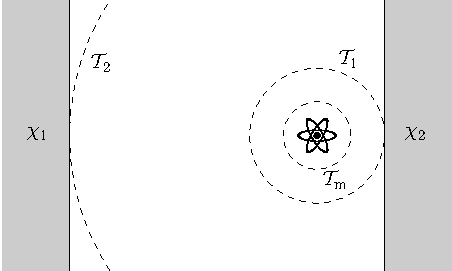
\includegraphics[width=0.5\linewidth]{fig/int-by-parts-gen}
  \caption[Thresholds for partial averaging for atom between two bodies]
  {Thresholds for partial averaging for atom between two dielectric bodies with susceptibilities $\chi_1$ and $\chi_2$.
    The dashed circles show the typical scales of paths at some important path times.
    The extent of the averaging is given by $\cT_m$.  The first path time when paths touch one body is 
    $\cT_1$. This is much smaller than the path time to touch \emph{both} bodies $\cT_2$.  
    These considerations also apply to the calculating stress-energy tensor close to one body.}
  \label{fig:int-by-parts-gen}
\end{figure}

However, if there is an analytical expression path integral near one surface, 
the further partial averaging is possible.  
In such a two body geometry, the renormalized two-body integration energy would lead to a function $\Phi$ specified by 
\begin{align}
  \Phi[x(t)] =& \Big(e^{-\int_0^\cT dt\,\{V_1[x(t)] +V_2[x(t)]\}} -e^{-\int_0^\cT dt\,\{V_1(x_0) +V_2(x_0)\}   }\Big)\nonumber\\
 & -\Big( e^{-\int_0^\cT dt\,V_1[x(t)]   } -e^{-\int_0^\cT dt\,V_1(x_0)   }\Big)-\Big( e^{-\int_0^\cT dt\,V_2[x(t)]   } -e^{-\int_0^\cT dt\,V_2(x_0)   }\Big),
\end{align}
where $V_1$ and $V_2$ describe the two surfaces.
For points much closer to one body, and for short times $\Delta \cT$, then the total potential 
can be approximated based on the nearest body 
\begin{equation}
  \Biglinklangle e^{-\int_0^{\Delta\cT}dt\,\{ V_1[x(t)]+ V_2[x(t)]\}}\Biglinkrangle \approx
  \Biglinklangle e^{-\int_0^{\Delta\cT}dt\,\{ V_2[x(t)]\}}\Biglinkrangle,
\end{equation}
where the presence of the far body can be ignored for short times.  
The partial averaging can be carried out by using the fact that the path integral is a propagator for the diffusion equation. 
The path-integral between two points $x_j$, $x_{j+1}$, interacting with a potential $V(x)$,
\begin{equation}
  U(x_j,x_{j+1},t):= \frac{e^{-(x_j-x_{j+1}^2/(2t)}}{\sqrt{2\pi t}} 
  \bigglinklangle e^{-\int_0^t dt' V[x(t')] }\bigglinkrangle_{x_j\rightarrow x_{j+1}},
\end{equation}
obeys the composition law,
\begin{equation}
  \int dx_j\, U(x_{j-1},x_{j},t_1)U(x_{j},x_{j+1},t_2) = U(x_{j-1},x_{j+1},t_1+t_2).
\end{equation}
So if such a potential $V$, and a closed solution can be found, then the partial averaging can be 
carried out to a threshold $\cT_m$ where the analytical path integral is no longer an acceptable approximation
to the true solution for multiple bodies.  
This could happen either due to the presence of multiple bodies, or the path exploring a region where
the geometry differs from that assumed in the analytical expression.  

After the partial averaging, the derivatives can be carried out, with the result
\begin{align}
  \partial_0^nI(x_0)&=\biggdlangle
  \partial_0^n [U(x_0,x_m,\cT_m) U(x_0,x_{N-m},\cT_m]\prod_{j=m}^{N-m-1}U(x_{j+1},x_j,\Delta \cT)
   \biggdrangle.
\end{align}
In this case, the derivatives act on the whole propagator , rather than just the Gaussian parts.  
This could be applied using the Dirichlet solution to the path integral for evaluating the 
stress-energy tensor (as was studied in Ref.~\cite{Schafer2016}).

\subsection{Results: TM Casimir  and Casimir--Polder Energies for Planar Geometries}

Figure~\ref{fig:eff_TM_atom_wall} plots the numerical results for the efficiency $\eta\subTM$
against the analytical expression~(\ref{eq:etaTM}).  The numerical results 
were collected using the preceding methods using birth-death path swarms to generate paths.
The path times were sampled  from Eq.~(\ref{eq:expT}), and the derivatives in Eq.~(\ref{eq:TM_Casimir_Polder})
were evaluated using the Gaussian partial averaging. 

\begin{figure}
\centering
  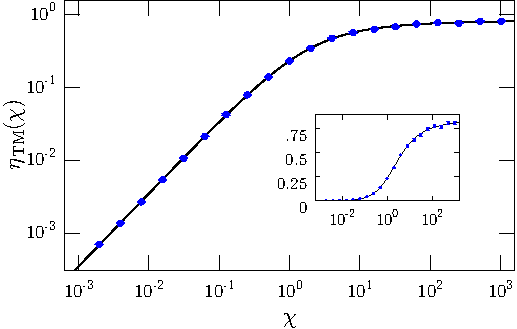
\includegraphics[width=0.8\textwidth]{fig/numerics/eff_TM_atom_wall}
  \caption[Numerical TM Casimir--Polder Efficiency]{Numerically computed TM Casimir--Polder Efficiency for Atom-Plane, 
    for $10^9$ paths, with $N=10^3$ points per path.  Birth-death method was used for path generation, and partial averaging was
  used for derivatives.}
  \label{fig:eff_TM_atom_wall}
\end{figure}

\begin{figure}
\centering
  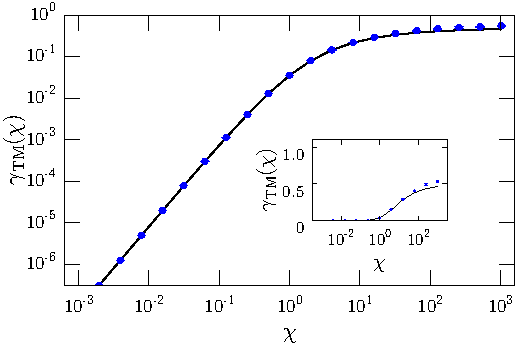
\includegraphics[width=0.8\textwidth]{fig/numerics/eff_TM_2wall}
  \caption[Numerical TM Casimir Efficiency]{Numerically computed TM Casimir Efficiency for Plane-Plane.
    for $N=200$, with $4.8\times 10^8$ trajectories.}
  \label{fig:eff_TM_2wall}
\end{figure}

The error bars are obviously much larger than their TE counterparts.
The length of the path $N$ is also smaller.
Larger paths take much longer to simulate, since there is more branching.  
Attempts to move to larger $N$ have run into very large numerical fluctuations.  
In the TE case, the convergence was found to improve as $N$ was increased, 
since the systematic error decreased.    
In the TM case, the decreased systematic error from larger $N$ conflicts with the growing
numerical fluctuations.  Of course, the numerical fluctuations can be mitigated by more averaging.
In addition, each susceptibility $\chi$ is simulated individually, since the branching in the birth-death
depends on the value of $\Xi$.  

Figure~\ref{fig:eff_TM_2wall} shows the numerically computed efficiency $\gamma\subTM$ for 
two planar dielectrics.  The agreement is not good in this case.  At large coupling, the error bars do not 
overlap with the analytical solution.
This may be down to the very small $N$ used in this calculation ($N=200$), which would lead
to a large systematic error.  Surprisingly, the TM Casimir results seem to be biased above the 
expected result.  

Sampling from the exponential path time distribution~(\ref{eq:expT}) 
is essential for the renormalized two-body TM Casimir energy.
Once paths are large enough to contribute to the energy, they are guaranteed to have intersected both 
bodies.  As a result, the intersection path time of the fiducial path with the surface has little bearing on when
the resulting path swarm would contribute.  For example, the fiducial path might have started next to 
one surface, and branched immediately.  The fiducial path might extend far more in one direction, 
and only intersect the second body at much later times than the new path.  Sampling the path time
based on when the fiducial path intersects the body would miss that contribution.
This suggests that the path time for the birth-death path swarm is best sampled from the 
ensemble average estimate of when a path will contact the surface.  

The renormalized Casimir energy has an additional problem.  As currently implemented,
the starting position for paths is randomly sampled from Eq.~(\ref{eq:xPower_law}).  As already
alluded to, the paths can start close to one surface, and spawn a number of child paths
immediately.  However, these paths are not guaranteed to intersect both bodies, and thus a
large number of them contribute zero to the renormalized path integral.  This
wastes a lot of computational effort on computing zero.
One possible improvement to this method is to explicitly force the path to touch both bodies.  
This would be another form of importance sampling, since only paths that touch both bodies 
will actually contribute to the path integral.    


\section{Frequency Sampling}


% \subsection{Path Construction Revisited: Path-Pinning as Importance Sampling}

% In the curvature numerics, the forces emerged from paths constrained to touch the surfaces 
% of the interacting bodies.  While this is a necessity for forces, constrained paths can also be used
% to compute Casimir energies.
% Although the Casimir energies do not require such constraints, the renormalized 
% integrand is only non-zero for paths that touch both surfaces.
% This suggest using paths constrained to touch both surfaces by construction.  This is a form of importance
% sampling, beyond what is suggested by the Gaussian measure of the worldline path integral.
% We would construct paths that are constrained to touch both surfaces, and correct for this modification
% to the path integral.  In the TM Casimir energy, this is very useful, since the birth-death method 
% causes many paths to be created, and ideally most of these new paths would also contribute to the path 
% integral.  
% In the absence of such a bias, a large number of paths are created near one surface, and if these paths
% do not intersect the other body, a large amount of computational effort is wasted.  

% Consider a Gaussian path integral,
% \begin{equation}
%   I_k=\int \frac{d\cT}{(2\pi)^{D/2}\cT^{1+D/2}}\int d\vect{x}\, f(\vect{x})P(\vect{x}),
% \end{equation}
% where $f$ is some function of the whole path that is only non-zero if the path enters a given region.
% The $D-1$-dimensional probability density is given by,
% \begin{equation}
%   P(\{\vect{x}\}) = (2\pi\cT)^{(D-1)/2}\prod_{k=0}^{N-1} \frac{1}{(2\pi\Delta\cT)^{(D-1)/2}}e^{-(\vect{x}_{k+1}-\vect{x}_k)^2/(2\Delta\cT)},
% \end{equation}
% Instead of just taking $P$ as the probability density, let us consider using $Q=P(\vect{x})|_{x_k=d}$,
% where one point is fixed on the surface of the region
% \begin{align}
%   Q(\{\vect{x}\}) =& (2\pi\cT)^{(D-1)/2}\cN_Q^{-1}\prod_{j=0}^{N-1}
%  \frac{1}{(2\pi\Delta\cT)^{(D-1)/2}}e^{-(\vect{x}_{j+1}-\vect{x}_j)^2/(2\Delta\cT)}\bigg|_{x_k=\vect{d}},
%   \end{align}
%   where the normalization constant is
% \begin{equation}
% \cN_Q=\bigg[\frac{N^2}{2\pi k(N-k)\cT}\bigg]^{(D-1)/2}
% e^{-N^2(\vect{d}-\vect{x}_0)^2/[2k(N-k)\cT]}
% \end{equation}
% The ratio of the probability densities is 
% \begin{align}
%   \frac{P}{Q} &= \cN_Q\frac{\exp\left[-\frac{(\vect{x}_{k-1}-\vect{x}_k)^2}{2\Delta \cT}
%       -\frac{(\vect{x}_{k}-\vect{x}_{k+1})^2}{2\Delta \cT}\right]}
%   {\exp\left[-\frac{(\vect{x}_{k-1}-\vect{d})^2}{2\Delta \cT}
%       -\frac{(\vect{d}-\vect{x}_{k+1})^2}{2\Delta \cT}\right]}
% %  \\  &
% = \cN_Q\exp\left[-\frac{(\vect{x}_{k}-\bar{\vect{x}})^2}{\Delta \cT}
%       +\frac{(\vect{d}-\bar{\vect{x}})^2}{\Delta \cT}\right].
% \end{align}
% % Note that the paths are constructed to ensure $\vect{x}_0\rightarrow\vect{d}$.  There is still one 
% % remaining integral which can also be sampled from in determining the integrand, but this sampled $\vect{x}_k$
% % does not alter the path.  

% The resulting integrand could be built up from Monte Carlo samples 
% \begin{equation}
%   I_k = \int \frac{d\cT}{(2\pi)^{D/2}\cT^{1+D/2}}\int d\vect{x}_k\, \cN_Q e^{-\frac{(\vect{x}_{k}-\bar{\vect{x}})^2}{\Delta \cT}
%       +\frac{(\vect{d}-\bar{\vect{x}})^2}{\Delta \cT}} f(\vect{x})Q(\vect{x})
% \end{equation}
% The normalization $\cN_Q$ can be used to sample the times, with $s=D/2$ and $\cT_0=N^2|\vect{d-x}_0|^2/[2k(N-k)]$ as the distribution
% parameters.
% The remaining $\vect{x}_k$ integral can be evaluated by using the Gaussian.
% However, those sampled values of $\vect{x}_k$ are not the path values, rather they are sampled after
% the path is constructed subject to the pinning requirement.    
% The appropriate integrand for Monte carlo in pinned paths, $\vect{x}_k$ and times $\cT$ is 
% \begin{align}
%   I_k &= \dlangle \frac{\Gamma[D/2]}{\cT_0^{D/2}}\bigg(\frac{N}{2\pi k (N-k)\Delta\cT}\bigg)^{(D-1)/2}
%   (\pi \Delta\cT)^{(D-1)/2} e^{\frac{(\vect{d}-\bar{\vect{x}})^2}{\Delta \cT}} f(\vect{x})\drangle_{\{\vect{x}\}',\vect{x}_k,\cT}\nonumber\\
%    % &= \dlangle \Gamma[D/2] \left(\frac{2k(N-k)}{N^2\vect{|d-x_0|}^2}\right)^{D/2} \frac{N^{n/2}}{[2k(N-k)]^{n/2}}
%    %  e^{\frac{(\vect{d}-\bar{\vect{x}})^2}{\Delta \cT}} f(\vect{x})\drangle_{\{\vect{x}\}',\vect{x}_k}\\
%    &= \dlangle \Gamma[D/2] \frac{[2k(N-k)]^{(D-n)/2}}{N^{D-n/2}\vect{|d-x_0|}^D}   
%    e^{\frac{(\vect{d}-\bar{\vect{x}})^2}{\Delta \cT}} f(\vect{x})\drangle_{\{\vect{x}\}',\vect{x}_k,\cT}.
%  \end{align}

% Of course, if the pinned point is also integrated over (such as the transverse dimensions for a planar medium),
%  then a different distance dependence.
%   In that case, only one dimension remains to be evaluated in the path integral,
% % \begin{align}
% %   I   &= \dlangle \Gamma[D/2] \frac{[2k(N-k)]^{(D-1)/2}}{N^{D-1/2}|d-x_0|^D}   
% %   e^{\frac{(\vect{d}-\bar{\vect{x}})^2}{\Delta \cT}} f(\vect{x})\drangle_{\{\vect{x}\}',\vect{x}_k,\cT}.
% % \end{align}
% The result can be written out explicitly for $D=4$
% \begin{align}
%   I   &= \dlangle  \frac{[2k(N-k)]^{3/2}}{N^{2}N^{3/2}|d-x_0|^4}   
%   e^{\frac{(\vect{d}-\bar{\vect{x}})^2}{\Delta \cT}} f(\vect{x})\drangle_{\{\vect{x}\}',\vect{x}_k,\cT}.
% \end{align}

% The above development fixed one particular index $k$.  This index $k$ can also be sampled over to vary
% which points are pinned to the surface.  We propose using $P_k= 6 k(N-k)/N^2$, as this is simple to sample
% from and is not too sharply peaked around $k=N/2$.

%%% Local Variables: 
%%% mode: latex
%%% TeX-master: "thesis_master"
%%% End: 
